\section{Introduction}
\label{sec:intro}

% Intro to Adaptive Analysis

The computational complexity of most problems is studied in the worst
case over instances of fixed size $n$, for $n$ asymptotically tending
to infinity. This approach was refined for NP-difficult problems under
the term ``parameterized
complexity''~\cite{2006-BOOK-ParameterizedComplexityTheory-FlumGrohe},
for polynomial problems under the term ``Adaptive
Algorithms''~\cite{1992-ACMCS-ASurveyOfAdaptiveSortingAlgorithms-EstivillCastroWood,1992-ACJ-AnOverviewOfAdaptiveSorting-MoffatPetersson},
and more simply for data encodings under the term of ``Data
Compression''~\cite{2013-TCS-OnCompressingPermutationsAndAdaptiveSorting-BarbayNavarro},
for a wide range of problems and data types.
Such a variety of results has motivated various tentative to classify
them, in the context of NP-hard problems with a theory of Fixed
Parameter
Tractability~\cite{2006-BOOK-ParameterizedComplexityTheory-FlumGrohe},
and in the context of \textsc{Sorting} in the comparison model with a theory of
reduction between
parameters~\cite{1995-DAM-AFrameworkForAdaptiveSorting-PeterssonMoffat}.

% Examples of Results and Classification in Adaptive Analysis

In the context of the ``Adaptive Analysis of Algorithms'', we
introduce two other perspectives from which to classify algorithms and
data structures: those taking advantage of the \emph{input order}
(e.g., disorder measures for \textsc{Sorting}
permutations~\cite{1992-ACJ-AnOverviewOfAdaptiveSorting-MoffatPetersson,1992-ACMCS-ASurveyOfAdaptiveSortingAlgorithms-EstivillCastroWood},
decomposition in simple subchains for \textsc{Convex
  Hull}~\cite{2002-SWAT-AdaptiveAlgorithmsForConstructingConvexHullsAndTriangulationsOfPolygonalChains-LevcopoulosLingasMitchell})
and those taking advantage of the \emph{input structure} (e.g., output
sensitive
algorithms~\cite{1986-JCom-TheUltimatePlanarConvexHullAlgorithm-KirkpatrickSeidel}
and input order oblivious instance
optimality~\cite{2009-FOCS-InstanceOptimalGeometricAlgorithms-AfshaniBarbayChan}
both for \textsc{Convex Hull}).

By ``\emph{input order}'' we mean algorithms taking advantage of the order
of the input, for example, taking advantage of the order of the values
in a sequence of numbers or of the order in which the points are given
in a polygonal chain.
% input order sorting
Concerning the \textsc{Sorting} problem, as early as 1973,
Knuth~\cite{1973-BOOK-TheArtOfComputerProgrammingVol3-Knuth} described
a variant of the algorithm {\tt{MergeSort}} that sorts an array
$\mathcal{A}$ using a prepossessing step taking linear time to detect
maximal sorted subblocks, called \emph{runs}, in $\mathcal{A}$.
Takaoka~\cite{2009-Chapter-PartialSolutionAndEntropy-Takaoka}
described a new sorting algorithm that optimally takes advantage of
the distribution of the sizes of the runs in the array $\mathcal{A}$,
which yields a time complexity within
$O(n(1+\mathcal{H}(r_1, \dots, r_{\rho}))) \subseteq
O(n(1{+}\log{\rho})) \subseteq O(n\log{n})$, where $\rho$ is the
number of runs in $\mathcal{A}$ and $r_1, \dots, r_{\rho}$ are the
sizes of the $\rho$ \emph{runs} (such that $\sum_{i=1}^\rho {r_i}=n$),
respectively. Takaoka measures the ``difficulty'' of the instance in
terms of the ``input order'' by the entropy function
$\mathcal{H}(r_1, \dots, r_\sigma) =
\sum_{i=1}^\sigma{\frac{r_i}{n}}\log{\frac{n}{r_i}}$. These results
take advantage of the order of the values in the input i.e., the input
order.
% input order convex hull
Considering the computation of the {\sc{Convex Hull}} in the plane,
Levcopoulos et
al.~\cite{2002-SWAT-AdaptiveAlgorithmsForConstructingConvexHullsAndTriangulationsOfPolygonalChains-LevcopoulosLingasMitchell}
described a divide-and-conquer algorithm for computing the {\sc{Convex
    Hull}} of a polygonal chain. They measured the complexity of this
algorithm in terms of the minimum number of simple subchains $\kappa$
into which the chain can be cut.  They showed that the time complexity
of this algorithm is within
$O(n(1{+}\log{\kappa})) \subseteq O(n\log{n})$. This result takes
advantage of the order in which the points are given i.e., the input
order.

By ``\emph{input structure}'' we mean algorithms taking advantage of the
structure of the instance, for example, taking advantage of the
frequencies of the values in a multiset or of the relative positions
of the points in a set of planar points.
% Input structure sorting
Concerning the {\sc{Sorting}} problem, as early as 1976, Munro and
Spira~\cite{1976-JComp-SortingAndSearchingInMultisets-MunroSpira}
considered the task of sorting a multiset
$\mathcal{M}=\{x_1, \dots, x_n\}$ of $n$ real numbers with $\sigma$ distinct
values, of multiplicities $m_1, \dots, m_\sigma$ (such that
$\sum_{i=1}^\sigma {m_i}=n$), respectively. They showed that adding
counters to various classical algorithms
\begin{INUTILE}
  (among which the divide-and-conquer based algorithm
  {\tt{MergeSort}})
\end{INUTILE}
yields a time complexity within
$O(n(1+\mathcal{H}(m_1, \dots, m_\sigma))) \subseteq
O(n(1{+}\log{\sigma})) \subseteq O(n\log{n})$ for sorting $\mathcal{M}$. This result takes advantage of the frequencies of the values
i.e., the structure of the instance.
% Input order convex hull
Considering the problem of computing the {\sc{Convex Hull}}, Kirkpatrick and Seidel~\cite{1986-JCom-TheUltimatePlanarConvexHullAlgorithm-KirkpatrickSeidel} described an algorithm to compute the {\sc{Convex Hull}} of a set of $n$ planar points in time within $O(n(1+\log h))\subseteq O(n\log n)$, where $h$ is the number of vertices in the {\sc{Convex Hull}}.
\begin{INUTILE}
  The algorithm relies on a variation of the divide-and-conquer
  paradigm, which they call the ``Marriage-Before-Conquest''
  principle.
\end{INUTILE}
Afshani et al.~\cite{2009-FOCS-InstanceOptimalGeometricAlgorithms-AfshaniBarbayChan} refined the complexity analysis of this algorithm to within $O(n(1+{\cal H}(n_1,\ldots,n_h)))\subseteq O(n(1{+}\log h)) \subseteq O(n\log{n})$, where $n_1, \dots, n_h$ are the sizes of a partition of the input, such that every element of the partition is a singleton or can be enclosed by a triangle whose interior is completely below the upper hull of the set, and ${\cal H}(n_1,\ldots,n_h)$ has the minimum possible value (minimum entropy of the distribution of the points into a certificate of the instance). This result takes advantage of the positions of the points i.e., the structure of the instance.

% Hypothesis

\paragraph{Hypothesis:}~\\ Is it possible to combine both categories of
techniques into a single algorithm taking advantage of the input order
and structure in a synergistic way?~\\

% Conclusion

Through the study of the sorting of multisets according to the
potential ``easiness'' in both the order and the values in the
multiset, in Section~\ref{sec:syn-sort} we show an example of the
difficulty of combining both into a single hybrid synergistic algorithmic
technique. 
This improves upon both algorithms from Munro and
Spira~\cite{1976-JComp-SortingAndSearchingInMultisets-MunroSpira} and
Takaoka~\cite{2009-Chapter-PartialSolutionAndEntropy-Takaoka}.
%
Through the study of the support of \texttt{rank} and \texttt{select}
queries on multisets according to the potential ``easiness'' in both
the order and the values in the queries themselves (in addition to the
potential easiness in the data being queried), in
Section~\ref{sec:multiselect} and Section~\ref{sec:dds} we extend the
results to the context of \textsc{MultiSelection} and \textsc{Deferred
  Data Structures}. This improves upon \textsc{MultiSelection}
algorithms from Dobkin and
Munro~\cite{1981-JACM-OptimalTimeMinimalSpaceSelectionAlgorithms-DobkinMunro}
and Kaligosi et
al.~\cite{2005-ICALP-TowardsOptimalMultopleSelection-KaligosiMehlhornMunroSanders}
and improve upon \textsc{Deferred Data
  Structures} results from Barbay et al.'s~\cite{2016-JDA-NearOptimalOnlineMultiselectionInInternalAndExternalMemory-BarbayGuptaRaoSorenson}
by adding 3 new measures of difficulty (input order, input structure
and query order) to the single one previously considered (query
structure). These combinations yield a better
understanding of the problems and more efficient solutions which we
hope to extend to other problems (described in Sections~\ref{sec:compressed},~\ref{sec:maxima} and~\ref{sec:hull}).

\section{Sorting Solutions}
\label{sec:sort}

We review in Section~\ref{sec:back} the algorithms \texttt{MergeSort
  with Counters} described by Munro and
Spira~\cite{1976-JComp-SortingAndSearchingInMultisets-MunroSpira} and
\texttt{Minimal MergeSort} described by
Takaoka~\cite{2009-Chapter-PartialSolutionAndEntropy-Takaoka}, which each
takes advantage of distinct features in the input. In Section
\ref{sec:syn-sort}, we describe two synergistic \textsc{Sorting}
algorithms, which never perform worse than a constant factor than \texttt{MergeSort with
  Counters} and \texttt{Minimal MergeSort}, and perform much better on
some large classes of instances by taking advantage of both the order
and the structure in the input, in a synergistic way. In
Section~\ref{sec:multiselect}, we generalize one of the algorithm
described in Section~\ref{sec:syn-sort} to an offline multiselection
algorithm that partially sorts a multiset according to the set of
\texttt{select} queries given as input. In the context where the
queries arrive one at the time (i.e., online), in
Section~\ref{sec:dds} we define two \textsc{Deferred Data Structures}
for answering online \texttt{rank} and \texttt{select} queries, both
inspired by the \texttt{MultiSelection} algorithm.

\subsection{Background}
\label{sec:back}

The algorithm \texttt{MergeSort with Counters} described by Munro and
Spira~\cite{1976-JComp-SortingAndSearchingInMultisets-MunroSpira} is
an adaptation of the traditional sorting algorithm \texttt{MergeSort}
that optimally takes advantage of the structure in the input when
sorting a multiset $\mathcal{M}$ of size $n$. The algorithm divides
$\mathcal{M}$ into two equal size parts, sorts both parts recursively,
and then merges the two sorted lists. When two elements of same value $v$ are
found, one is thrown away and a counter holding the number of occurrences
of $v$ is updated. Munro and Spira measure the
``difficulty'' of the instance in terms of the ``input structure'' by
the entropy function
$\mathcal{H}(m_1, \dots, m_\sigma) =
\sum_{i=1}^\sigma{\frac{m_i}{n}}\log{\frac{n}{m_i}}$.  The time
complexity of the algorithm is within
$O(n(1 + \mathcal{H}(m_1, \dots, m_\sigma))) \subseteq
O(n(1{+}\log{\sigma})) \subseteq O(n\log{n})$, where $\sigma$ is the
number of distinct elements in $\mathcal{M}$ and
$m_1, \dots, m_\sigma$ are the multiplicities of the $\sigma$ distinct
elements in $\mathcal{M}$ (such that $\sum_{i=1}^\sigma {m_i}=n$),
respectively.

The algorithm \texttt{Minimal MergeSort} described by
Takaoka~\cite{2009-Chapter-PartialSolutionAndEntropy-Takaoka}
optimally takes advantage of the local order in the input, as measured
by the decomposition into runs when sorting an array $\mathcal{A}$ of
size $n$.  The main idea is to detect the runs first and then merge
them pairwise\begin{LONG}, using a \texttt{MergeSort}-like
  step\end{LONG}. The runs are detected in linear time\begin{LONG} by
  a scanning process identifying the positions $i$ in $\mathcal{A}$
  such that $\mathcal{A}[i] > \mathcal{A}[i+1]$\end{LONG}. Merging the
two shortest runs at each step further reduces the number of
comparisons, making the running time of the merging process adaptive
to the entropy of the sequence of the sizes of the runs.  The merging
process is then represented by a tree with the shape of a
Huffman~\cite{1952-IRE-AMethodForTheInstructionOfMinimumRedundancyCodes-Huffman}
tree, built from the distribution of the sizes of the \emph{runs}.  If
the array $\mathcal{A}$ is formed by $\rho$ runs and
$r_1, \dots, r_{\rho}$ are the sizes of the $\rho$ runs (such that
$\sum_{i=1}^\rho {r_i}=n$), then the algorithm sorts $\mathcal{A}$ in
time within
$O(n(1+\mathcal{H}(r_1, \dots, r_{\rho}))) \subseteq
O(n(1{+}\log{\rho})) \subseteq O(n\log{n})$.

The algorithm \texttt{MergeSort with Counters} is incomparable with
the algorithm \texttt{Minimal MergeSort}, in the sense that neither
one performs always better than the other. Simple modifications and
combinations of these algorithms do not take full advantage of both
the order and structure in the input
(see~\cite{2016-ARXIV-SynergisticSortingAndDeferredDataStructuresOnMultiSets-BarbayOchoaSatty}
for detailed counter examples).

\subsection{Synergistic Sorting}
\label{sec:syn-sort}

In the following section we describe two sorting algorithms that take
the best advantage of both the order and structure
in the input all at once when sorting a multiset. The first one is a
straightforward application of previous results, while the second one
prepares the ground for the \textsc{MultiSelection} algorithm
(Section~\ref{sec:multiselect}) and the \textsc{Deferred Data
  Structures} (Section~\ref{sec:dds}), which take
advantage of the order and structure in the data
and of the order and structure in the queries.

\subsubsection{Sorting Algorithm \texttt{DLM
    Sort}}
\label{sec:dlm-sort}

In 2000, Demaine et
al.~\cite{2000-SODA-AdaptiveSetIntersectionsUnionsAndDifferences-DemaineLopezOrtizMunro}
described the algorithm \texttt{DLM Union}, an instance optimal
algorithm that computes the union of $\rho$ sorted sets.  The
algorithm scans the sets from left to right identifying blocks of
consecutive elements in the sets that are also consecutive in the
sorted union. The time complexity of the \texttt{DLM Union} algorithm
is measured in terms of the number and sizes of these blocks (see
Figure~\ref{fig:instance} where it is depicted an instance of the
\textsc{Set Union} problem); the sizes of these blocks are referred to
as \emph{gaps} in the analysis of the algorithm.
\begin{INUTILE}
  These blocks induce a partition $\pi$ of the output into intervals
  such that any singleton corresponds to a value that has multiplicity
  greater than $1$ in the input, and each other interval corresponds
  to a block as defined above. Each member $i$ of $\pi$ has a value
  $m_i$ associated with it: if the member $i$ of $\pi$ is a block,
  then $m_i$ is $1$, otherwise, if the member $i$ of $\pi$ is a
  singleton corresponding to a value of multiplicity $q$, then $m_i$
  is $q$.
%
  Let $\chi$ be the size of $\pi$.
%
  If the instance is formed by $\delta$ blocks of sizes
  $g_1, \dots, g_{\delta}$ such that these blocks induce a partition
  $\pi$ whose members have values $m_1, \dots, m_{\chi}$, we express
  the time complexity of the algorithm \texttt{DLM Union} as within
  $\Theta(\sum^{\delta}_{i=1}\log g_i +
  \sum^{\chi}_{i=1}\log{\binom{\rho}{m_i}})$.
\end{INUTILE}
%
Demaine et
al.~\cite{2000-SODA-AdaptiveSetIntersectionsUnionsAndDifferences-DemaineLopezOrtizMunro}
showed that the time complexity of the \texttt{DLM Union} algorithm is
within a constant factor of the complexity of any other algorithm
computing the union of these sorted sets (i.e., the algorithm is
instance optimal).

\begin{minipage}[c]{.45\textwidth}
  \centering
  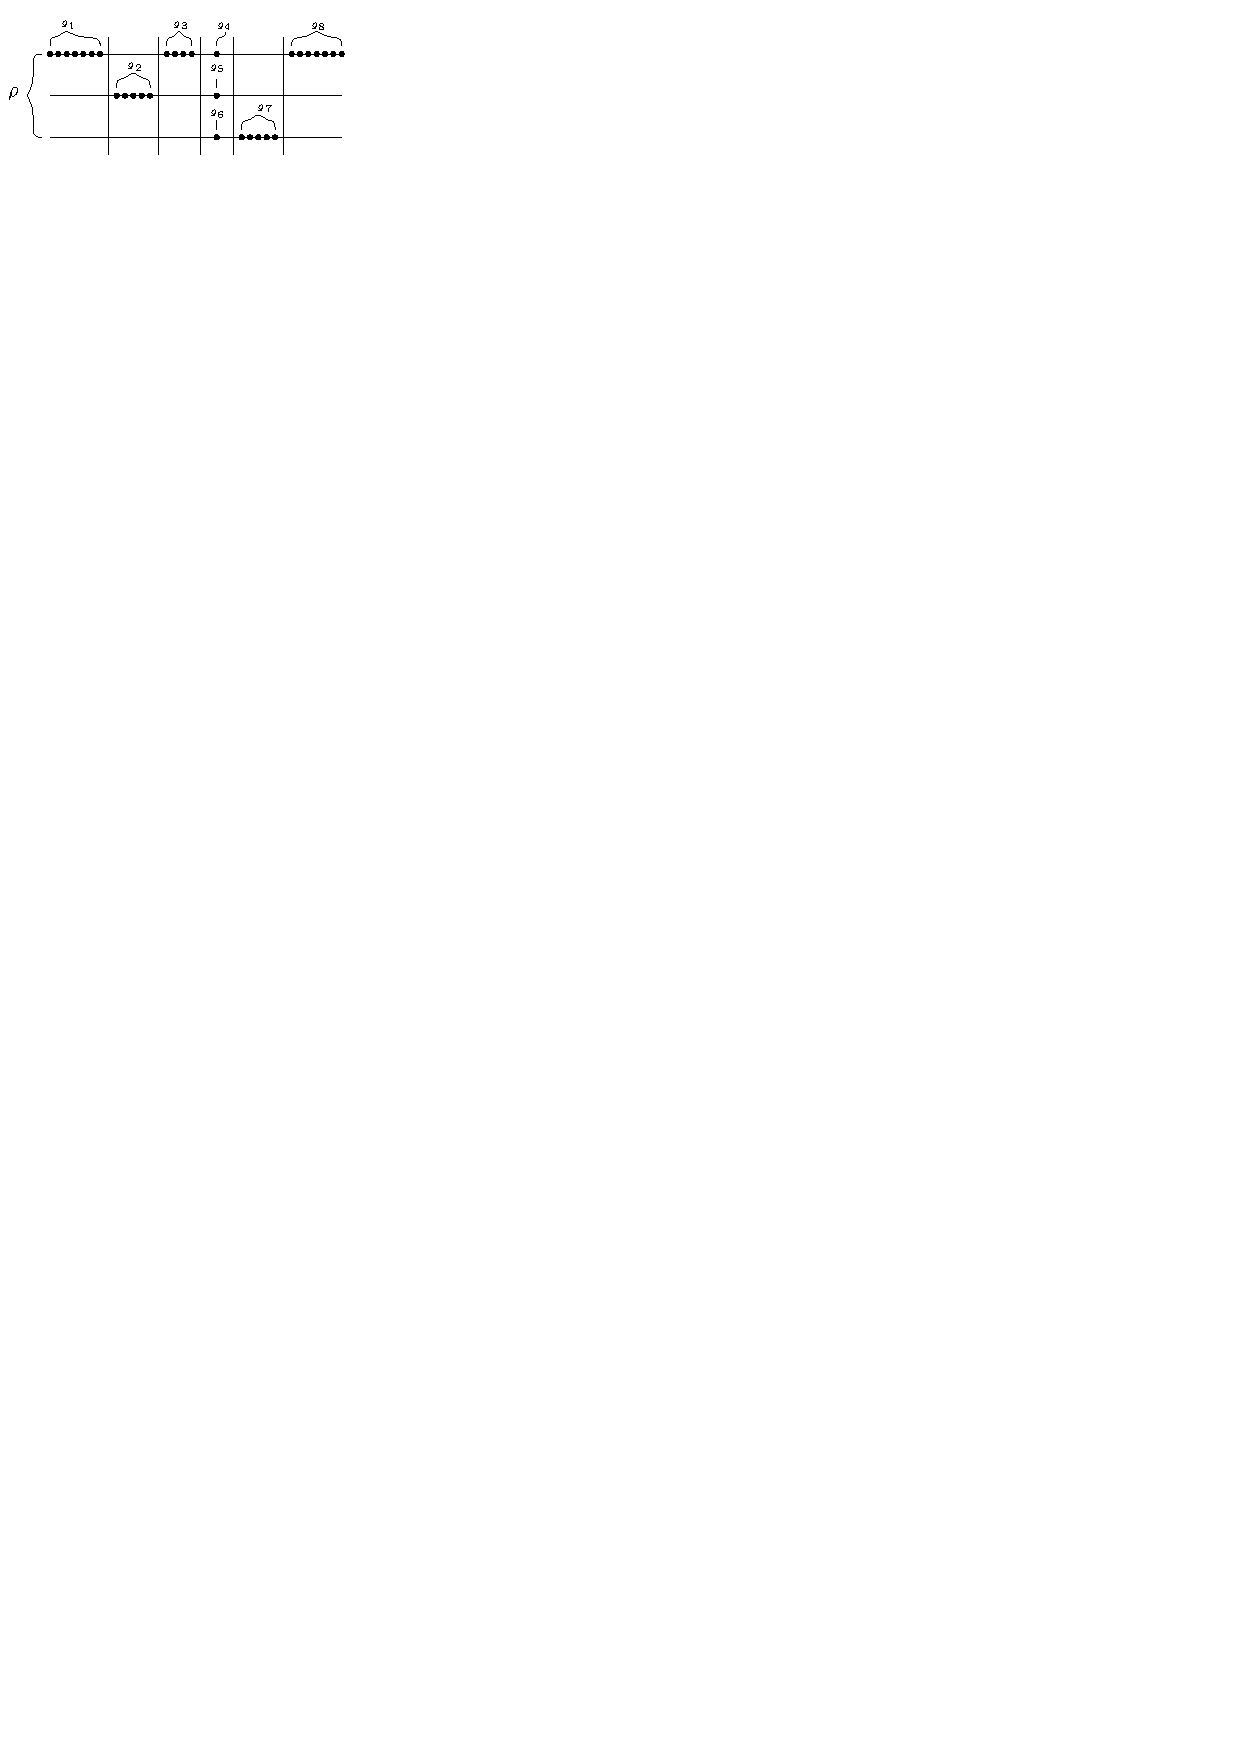
\includegraphics[scale=1.2]{union_instance1}
\end{minipage}\hfill
\begin{minipage}[c]{.45\textwidth}
  \captionof{figure}{An instance of the \textsc{Set Union} problem
    with $\rho=3$ sorted sets. In each set, the entry $\mathcal{A}[i]$
    is represented by a point of $x$-coordinate $\mathcal{A}[i]$. The
    blocks that form the sets are noted. The blocks $g_4,g_5$ and
    $g_6$ are of size 1 because they correspond to elements of equal
    value.}
  \label{fig:instance}
\end{minipage}

We adapt the \texttt{DLM Union} algorithm for sorting a multiset.  The
algorithm \texttt{DLM Sort} detects the runs first through a linear
scan and then applies the algorithm \texttt{DLM Union}. After that,
transforming the output of the union algorithm to yield the sorted
multiset takes only linear time.

\begin{INUTILE}
The following corollary follows from
our refined analysis above:

  \begin{corollary}
    Given a multiset $\mathcal{M}$ of size $n$ formed by $\rho$ runs
    and $\delta$ blocks of sizes $g_1, \dots, g_{\delta}$ such that
    these blocks induce a partition $\pi$ of size $\chi$ of the output
    whose members have values $m_1, \dots, m_{\chi}$, the algorithm
    {\tt{DLM Sort}} performs within
    $O(n + \sum^{\delta}_{i=1}\log g_i +
    \sum^{\chi}_{i=1}\log{\binom{\rho}{m_i}})$ data comparisons. This
    number of comparisons is optimal in the worst case over multisets
    of size $n$ formed by $\rho$ runs and $\delta$ blocks of sizes
    $g_1, \dots, g_{\delta}$ such that these blocks induce a partition
    $\pi$ of size $\chi$ of the output whose members have values
    $m_1, \dots, m_{\chi}$.
  \end{corollary}
\end{INUTILE}

While the algorithm \texttt{DLM Sort} sorts multisets taking the best
advantage of both the \emph{input order} and the \emph{input
  structure} in a synergistic way, it does not yield a
\textsc{MultiSelection} algorithm nor a \textsc{Deferred Data
  Structure}. In the following section we
describe another sorting algorithm that also optimally takes advantage
of the local order and structure in the input, but which is based on a
distinct paradigm, more suitable to such extensions.

\subsubsection{Sorting Algorithm {\texttt{Quick Synergy
      Sort}}}
\label{sec:qss}

Given a multiset $\mathcal{M}$, the algorithm \texttt{Quick Synergy
  Sort} identifies the \emph{runs} in linear time through a scanning
process. It computes a pivot $\mu$, which is the median
of the set formed by the middle elements of each run, and partitions
each \emph{run} by $\mu$. This partitioning process takes advantage of
the fact that the elements in each \emph{run} are already sorted. It
then recurses on the elements smaller than $\mu$ and on the elements
greater than $\mu$. (See Algorithm~\ref{alg:qss} for a more formal
description).

\begin{INUTILE}
  \begin{definition}[Median of the middles]
    Given a multiset $\mathcal{M}$ formed by runs, the ``\emph{median
      of the middles}'' is the median element of the set formed by the
    middle elements of each run.
  \end{definition}
\end{INUTILE}
\begin{algorithm} % enter the algorithm environment
  \caption{\texttt{Quick Synergy Sort}} % give the algorithm a caption
  \label{alg:qss} % and a label for \ref{} commands later in the document
  \begin{algorithmic}[1] % enter the algorithmic environment

    \REQUIRE{A multiset $\mathcal{M}$ of size $n$} \ENSURE{A sorted sequence of
      $\mathcal{M}$}

    \STATE Compute the $\rho$ runs of respective sizes
    $(r_i)_{i\in[1..\rho]}$ in $\mathcal{M}$ such that
    $\sum^{\rho}_{i=1} r_i = n$;
    \STATE Compute the median $\mu$ of
    the middles of the runs, note $j\in[1..\rho]$ the run containing
    $\mu$;
    \STATE Perform doubling searches for the value $\mu$ in all
    runs except the $j$-th, starting at both ends of the runs in
    parallel;
    \STATE Find the maximum $\max_\ell$ (minimum $\min_r$)
    among the elements smaller (resp., greater) than $\mu$ in all runs
    except the $j$-th;
    \STATE Perform doubling searches for the values
    $\max_\ell$ and $\min_r$ in the $j$-th run, starting at the
    position of $\mu$;
    \STATE Recurse on the elements smaller than o
    equal to $\max_\ell$ and on the elements greater than or equal to
    $\min_r$.
  \end{algorithmic}
\end{algorithm}

The number of data comparisons performed by the algorithm
\texttt{Quick Synergy Sort} is asymptotically the same as the number
of data comparisons performed by the algorithm \texttt{DLM Sort}
described in the previous section. Consequently, \texttt{Quick
  Synergy Sort} takes the best advantage of both the \emph{input order} and
the \emph{input structure} in a synergistic way.

Both algorithms \texttt{DLM Sort} and \texttt{Quick Synergy Sort}
perform much better than \texttt{MergeSort with Counters} and
\texttt{Minimal MergeSort} on large classes of instances, while
performing always asymptotically as good as them.

\begin{INUTILE}
  \begin{theorem}
    Let $\mathcal{M}$ be a multiset of size $n$ formed by $\rho$ runs
    and $\delta$ blocks of sizes $g_1, \dots, g_{\delta}$ such that
    these blocks induce a partition $\pi$ of the output of size $\chi$
    whose members have values $m_1, \dots, m_{\chi}$. The algorithm
    \texttt{Quick Synergy Sort} performs within
    $O(n + \sum^{\delta}_{i=1} \log g_i +
    \sum^{\chi}_{i=1}\log{\binom{\rho}{m_i}})$ data comparisons on
    $\mathcal{M}$. This number of comparisons is optimal in the worst
    case over multisets of size $n$ formed by $\rho$ runs and $\delta$
    blocks of sizes $g_1, \dots, g_{\delta}$ such that these blocks
    induce a partition $\pi$ of size $\chi$ of the output whose
    members have values $m_1, \dots, m_{\chi}$.
  \end{theorem}
\end{INUTILE}

Next, we generalize the algorithm \texttt{Quick Synergy Sort} to an
offline multiselection algorithm that partially sorts a multiset according to the set
of \texttt{select} queries given as input.

\subsection{MultiSelection Algorithm}
\label{sec:multiselect}

Given a linearly ordered multiset $\mathcal{M}$ and a sequence of
ranks $r_1, \dots, r_q$, a multiselection algorithm must answer the
queries \texttt{select}($r_1$), $\dots$, \texttt{select}($r_q$) in
$\mathcal{M}$, hence partially sorting $\mathcal{M}$.

Given a multiset $\mathcal{M}$ and a set of $q$ \texttt{select}
queries, the algorithm \texttt{Quick Synergy MultiSelection}
follows the same first steps as the algorithm \texttt{Quick Synergy
  Sort}. But once it has computed the ranks of all elements in the block that
contains the pivot $\mu$, it determines which \texttt{select} queries
correspond to elements smaller than or equal to $\max_\ell$ and which
ones correspond to elements greater than or equal to $\min_r$ (see
Algorithm~\ref{alg:qss} for the definitions of $\max_\ell$ and
$\min_r$). It then recurses on both sides.

We extend the notion of blocks to the context of partial sorting.
\begin{INUTILE}
  \begin{definition}[Pivot Blocks]
    Given a multiset $\mathcal{M}$ formed by $\rho$ runs and $\delta$
    blocks. The ``\emph{pivot blocks}'' are the blocks of
    $\mathcal{M}$ that contain the pivots and the elements of value
    equals to the pivots during the steps of the algorithm
    \texttt{Quick Synergy MultiSelection}.
  \end{definition}
\end{INUTILE}
In each run, between the blocks identifies by the algorithm and the
insertion ranks of the pivots, there are consecutive blocks that the
algorithm \texttt{Quick Synergy MultiSelection} has not identified as
separated blocks, because no doubling searches occurred inside them.
With this idea the results in Section~\ref{sec:syn-sort} can be
generalized to the more general problem of
\textsc{MultiSelection}. This refined result improves the analyses of
\textsc{MultiSelection} algorithms from Dobkin and
Munro~\cite{1981-JACM-OptimalTimeMinimalSpaceSelectionAlgorithms-DobkinMunro}
and Kaligosi et
al.~\cite{2005-ICALP-TowardsOptimalMultopleSelection-KaligosiMehlhornMunroSanders}.
 
\begin{INUTILE}
  \begin{definition}[Selection Blocks]
    Given the $i$-th run, formed of various blocks, and $q$
    \texttt{select} queries, the algorithm \texttt{Quick Synergy
      MultiSelection} computes $\xi$ pivots in the process of
    answering the $q$ queries. During the doubling searches, the
    algorithm \texttt{Quick Synergy MultiSelection} finds the
    insertion ranks of the $\xi$ pivots inside the $i$-th run. These
    positions determine a partition of size $\xi+1$ of the $i$-th run
    where each element of the partition is formed by consecutive
    blocks or is empty. We call the elements of this partition
    ``\emph{selection blocks}''. The set of all selection blocks
    include the set of all pivot blocks.
  \end{definition}

Using these definitions, we generalize the results in Section~\ref{sec:syn-sort} to the more general problem of \textsc{MultiSelection}.

\begin{theorem}\label{theo:qsms}
  Given a multiset $\mathcal{M}$ of size $n$ formed by $\rho$ runs and
  $\delta$ blocks; and $q$ offline \texttt{select} queries over
  $\mathcal{M}$ corresponding to elements of \texttt{ranks}
  $r_1, \dots, r_q$. The algorithm \texttt{Quick Synergy
    MultiSelection} computes $\xi$ pivots in the process of answering
  the $q$ queries. Let $s_1,\dots, s_{\beta}$ be the sizes of the
  $\beta$ selection blocks determined by these $\xi$ pivots in all
  runs. Let $m_1, \dots, m_\lambda$ be the numbers of pivot blocks
  corresponding to the values of the $\lambda$ pivots with
  multiplicity greater than 1, respectively.  Let
  $\rho_0, \dots, \rho_\xi$ be the sequence where $\rho_i$ is the
  number of runs that have elements with values between the pivots $i$
  and $i+1$ sorted by \texttt{ranks}, for $i\in[1..\xi]$.  The
  algorithm \texttt{Quick Synergy MultiSelection} answers the $q$
  \texttt{select} queries performing within
  $O(n + \sum^{\beta}_{i=1}\log{s_i} +
    \beta\log{\rho}-\sum^{\lambda}_{i=1}m_i\log{m_i} -
    \sum^{\xi}_{i=0}\rho_i\log{\rho_i}) \subseteq
  O(n\log{n} - \sum^{q}_{i=0}\Delta_i\log{\Delta_i})$ data
  comparisons, where $\Delta_i = r_{i+1} - r_i$, $r_0=0$ and
  $r_{q+1}=n$.
\end{theorem}
\end{INUTILE}

In the \textsc{MultiSelection} problem, the queries are given all at the same time (i.e.,
offline). In the context where they arrive one at the time (i.e., online), we define
two \textsc{Deferred Data Structures} for answering online
\texttt{rank} and \texttt{select} queries, both inspired by the algorithm
\texttt{Quick Synergy MultiSelection}.

\subsection{Deferred Data Structures for MultiSets}
\label{sec:dds}

We describe two \textsc{Deferred Data Structures} that answer a set of \texttt{rank} and \texttt{select} queries arriving one at the time over a multiset $\mathcal{M}$, progressively sorting $\mathcal{M}$.  
%
Both data structures take advantage of the order and structure in the input, and of the structure in the queries.
%
The first data structure is in the RAM model of computation, at the cost of not taking advantage of the order in which the queries are given. The second data structure is in the comparison model (a more constrained model) but does take advantage of the query order.

\subsubsection{Taking Advantage of  Order and Structure in the Input, but only of Structure in the Queries}

Given a multiset $\mathcal{M}$ of size $n$, the \textsc{RAM Deferred
  Data Structure} is composed of a bitvector $\mathcal{A}$ of size
$n$, in which we mark the elements in $\mathcal{M}$ that have been
computed as pivots by the algorithm when it answers the online
queries; a dynamic predecessor and successor structure $\mathcal{B}$
over the bitvector $\mathcal{A}$, which allows us to find the two
successive pivots between which the query fits; and for each pivot $p$
found, the data structure stores pointers to the insertion ranks of
$p$ in each run, to the beginning and end of the block $g$ to which
$p$ belongs, and to the position of $p$ inside $g$. The dynamic
predecessor and successor structure $\mathcal{B}$ requires the RAM
model of computation in order to answer \emph{predecessor and
  successor queries} in time within
$o(\log{n})$~\cite{2002-JCSS-OptimalBoundsForThePredecessorProblemAndRelatedProblems-BeameFich}.

\begin{INUTILE}
  \begin{theorem}\label{theo:online-ram}
    Consider a multiset $\mathcal{M}$ of size $n$ formed by $\rho$
    runs and $\delta$ blocks. The \textsc{RAM Deferred Data Structure}
    computes $\xi$ pivots in the process of answering $q$ online
    \texttt{rank} and \texttt{select} queries over $\mathcal{M}$. Let
    $s_1, \dots, s_{\beta}$ be the sizes of the $\beta$ selection
    blocks determined by these $\xi$ pivots in all runs. Let
    $m_1, \dots, m_\lambda$ be the numbers of pivot blocks
    \begin{LONG}
      among this selection blocks
    \end{LONG}
    corresponding to the values of the $\lambda$ pivots with
    multiplicity greater than 1, respectively.  Let
    $\rho_0, \dots, \rho_\xi$ be the sequence where $\rho_i$ is the
    number of runs that have elements with values between the pivots
    $i$ and $i+1$ sorted by \texttt{ranks}, for $i\in[1..\xi]$.  Let
    $u$ and $g_1, \dots, g_u $ be the number of \texttt{rank} queries
    and the sizes of the identified and searched blocks in the process
    of answering the $u$ \texttt{rank} queries, respectively. The
    \textsc{RAM Deferred Data Structure} answers these $q$ online
    \texttt{rank} and \texttt{select} queries in time within
    $O(n + \sum^{\beta}_{i=1}\log{s_i} + \beta\log{\rho} -
    \sum^{\lambda}_{i=1}m_i\log{m_i} -
    \sum^{\xi}_{i=0}\rho_i\log{\rho_i} + \xi\log\log{n} +
    u\log{n}\log\log{n} + \sum^{u}_{i=1}\log{g_i})$.
  \end{theorem}
\end{INUTILE}

The \textsc{RAM Deferred Data Structure} answers a new
\texttt{select}$(i)$ query by accessing in $\mathcal{A}$ the query
position $i$ to decide if the pivot was already computed. If not it finds
the nearest pivots to its left and right using the predecessor and
successor structure, $\mathcal{B}$. It then
applies the same steps as the algorithm \texttt{Quick Synergy
  MultiSelection} in order to answer the query. It updates the
bitvector $\mathcal{A}$ and the dynamic predecessor and successor
structure $\mathcal{B}$ whenever a new pivot is computed.

The \textsc{RAM Deferred Data Structure} answers a new
\texttt{rank}$(x)$ query by performing a sort of parallel binary
searches for the value $x$ at each run taking advantage of the pivots
that have been computed by the algorithm. The algorithm accesses the
position $\frac{n}{2}$ in $\mathcal{A}$ to decide if the pivot was
already computed. If not, then it finds the nearest
pivots to the left and right of the position $\frac{n}{2}$ using the
predecessor and successor structure, $\mathcal{B}$. Following the
pointers to the blocks that contain these pivots the algorithm decides
if $x$ is inside one of these blocks, to the right of the rightmost
block, to the left of the leftmost block, or between these two
blocks. In the last case, the algorithm applies the same steps as the
algorithm \texttt{Quick Synergy MultiSelection} in order to compute
the median $\mu$ of the middles and partitions the runs by
$\mu$. The algorithm then decides to which side $x$ belongs.

The \textsc{RAM Deferred Data Structure} takes advantage of the
structure in the queries and of the structure and order in the
input. Changing the order in the \texttt{rank} and \texttt{select}
queries does not affect the time complexity of the \textsc{RAM
  Deferred Data Structure}. Once the structure identifies the nearest
pivots to the left and right of the query positions, the steps of the
algorithms are the same as in the offline case
(Section~\ref{sec:multiselect}). We next describe a deferred data
structure taking advantage of the structure and order in the queries
and of the structure and order in the data.

\subsubsection{Taking Advantage of the Order and Structure in both the Input and the Queries}

To take advantage of the order in the queries, we introduce a
data structure that finds the nearest pivots to the left and to the
right of a position $p\in[1..n]$, while taking advantage of the
distance between the position of the last computed pivot and $p$. This
distance is measured in the number of computed pivots between the two
positions. For that we use a \emph{finger search
  tree}~\cite{1998-SODA-FingerSearchTreesWithConstantInsertionTime-Brodal}
which is a search tree maintaining \emph{fingers} (i.e., pointers) to
elements in the search tree. Finger search trees support efficient
updates and searches in the vicinity of the
fingers.

In the description of the \textsc{RAM Deferred Data Structure}, we
substitute the dynamic predecessor and successor structure
$\mathcal{B}$ by a finger search tree $\mathcal{F}_{\texttt{select}}$,
as described by
Brodal~\cite{1998-SODA-FingerSearchTreesWithConstantInsertionTime-Brodal}. Once
a block $g$ is identified, every element in $g$ is a valid pivot for
the rest of the elements in $\mathcal{M}$. In order to capture this
idea, we modify the structure $\mathcal{F}_{\texttt{select}}$ so that
it contains blocks (i.e., a sequence of consecutive values) instead of
singleton pivots. Each element in $\mathcal{F}_{\texttt{select}}$
points in $\mathcal{M}$ to the beginning and the end of the block $g$
that it represents and in each run to the position where the elements
of $g$ partition the run. This modification allows the structure to
answer \texttt{select} queries, taking advantage of the structure and
order in the queries and of the structure and order of the input
data. But in order to answer \texttt{rank} queries taking advantage of
the features in the queries and the input data, the structure needs
another finger search tree $\mathcal{F}_{\texttt{rank}}$. In
$\mathcal{F}_{\texttt{rank}}$ the structure stores for each block $g$
identified, the value of one of the elements in $g$, and pointers in
$\mathcal{M}$ to the beginning and the end of $g$. We name this
structure \textsc{Full-Synergistic Deferred Data Structure}.

\begin{INUTILE}
  \begin{theorem}\label{theo:finger}
    Consider a multiset $\mathcal{M}$ of size $n$ formed by $\rho$
    runs and $\delta$ blocks. The \textsc{Full-Synergistic Deferred
      Data Structure} identifies $\gamma$ blocks in the process of
    answering $q$ online \texttt{rank} and \texttt{select} queries
    over $\mathcal{M}$ corresponding to elements of \texttt{ranks}
    $r_1, \dots, r_q$. Let $s_1, \dots, s_{\beta}$ be the sizes of the
    $\beta$ selection blocks determined by the $\gamma$ blocks in all
    runs.  Let $m_1, \dots, m_\lambda$ be the numbers of pivot blocks
    \begin{LONG}
      among this selection blocks
    \end{LONG}
    corresponding to the values of the $\lambda$ pivots with
    multiplicity greater than 1, respectively.  Let
    $\rho_0, \dots, \rho_\xi$ be the sequence where $\rho_i$ is the
    number of runs that have elements with values between the pivots
    $i$ and $i+1$ sorted by \texttt{ranks}, for $i\in[1..\xi]$.  Let
    $d_1, \dots, d_{q-1}$ be the sequence where $d_j$ is the number of
    identified blocks between the block that answers the $j-1$-th
    query and the one that answers the $j$-th query before starting
    the steps to answer the $j$-th query, for $j\in[2..q]$. Let $u$
    and $g_1, \dots, g_u $ be the number of \texttt{rank} queries and
    the sizes of the identified and searched blocks in the process of
    answering the $u$ \texttt{rank} queries, respectively. The
    \textsc{Full-Synergistic Deferred Data Structure} answers the $q$
    online
    \begin{LONG}
      \texttt{rank} and \texttt{select}
    \end{LONG}
    queries performing within
    $O(n + \sum^{\beta}_{i=1}\log{s_i} + \beta\log{\rho} -
    \sum^{\lambda}_{i=1}m_i\log{m_i} -
    \sum^{\xi}_{i=0}\rho_i\log{\rho_i} + \sum^{q-1}_{i=1}\log{d_i} +
    \sum^{u}_{i=1}\log{g_i}) \subseteq O\left(n\log{n} -
      \sum^{q}_{i=0}\Delta_i\log{\Delta_i} + q\log{n}\right)$ data
    comparisons, where $\Delta_i = r_{i+1} - r_i$, $r_0=0$ and
    $r_{q+1}=n$.
  \end{theorem}
\end{INUTILE}

The \textsc{Full-Synergistic Deferred Data Structure} improve upon
\textsc{Deferred Data Structures} results from Barbay et
al.'s~\cite{2016-JDA-NearOptimalOnlineMultiselectionInInternalAndExternalMemory-BarbayGuptaRaoSorenson}
by adding 3 new measures of difficulty (input order, input structure
and query order) to the single one previously considered (query
structure).

Next, we describe three problems susceptible to combinations of input
order and input structure techniques.

\section{Compressed Data Structures}
\label{sec:compressed}

Consider an array ${\mathcal{A}}[1..n]$ of $n$ comparable objects. A \emph{Range
  Minimum
  Query}~\cite{1993-SICOMP-RecursiveStarTreeParallelDataStructure-BerkmanVishkin}
consists of a pair of integers $i$ and $j$ such that
$1\le i\le j\le n$, and is answered by
\texttt{RMinQ}$_{\mathcal{A}}(i,j)$, the leftmost position of a
minimum in $\mathcal{A}[i..j]$. Such queries have a wide range of
applications in various data structures and algorithms, including text
indexing~\cite{2009-TCS-FasterEntropyBoundedCompressedSuffixTrees-FischerMakinenNavarro},
pattern
matching~\cite{2008-STACS-ImprovedAlgorithmsForTheRangeNextValueProblemAndApplications-CrochemoreIliopoulosKubicaRahmanWalen},
and more elaborate kinds of range
queries~\cite{2004-ISAAC-OnTheRangeMaximumSumSegmentQueryProblem-ChenChao}.

%%% RMQs in presence of Repetitions.

If the array $\mathcal{A}$ is formed by repeated elements, then it is possible
to define more specific queries related to the
\texttt{RMinQ}$_{\mathcal{A}}(i,j)$ operation. The \emph{Range
  Leftmost Minimum Queries} (\texttt{RLMinQ}$_{\mathcal{A}}(i,j)$),
\emph{Range Rightmost Minimum Queries}
(\texttt{RRMinQ}$_{\mathcal{A}}(i)$) and \emph{Range k-th Minimum
  Query} (\texttt{RkMinQ}$_{\mathcal{A}}(i,j)$) return, given $m$
elements of minimum values of ranks $r_1, \dots, r_m$ in the range
${\mathcal{A}}[i..j]$, $r_1$, $r_m$ and $r_k$, respectively.
%%% PSVs
Similar kind of queries are \emph{Previous Smaller Value}
\texttt{PSV}$_{\mathcal{A}}(i)$ and \emph{Previous Larger Value}
\texttt{PLV}$_{\mathcal{A}}(i)$, which return the position of the nearest
smaller/larger value among ${\mathcal{A}}[1..i]$, by analogy the operations
\emph{Next Smaller Value} \texttt{NSV}$_{\mathcal{A}}(i)$ and \emph{Next Larger Value}
\texttt{NLV}$_{\mathcal{A}}(i)$ can be defined.

Fischer~\cite{2010-LATIN-OptimalSuccinctnessForRangeMinimumQueries-Fischer}
described a non-systematic succinct index (which does not access the
original data when answering queries) using $2n+o(n)$ bits and
supporting \texttt{RMinQ}$_{\mathcal{A}}(i,j)$ in zero accesses to
$\mathcal{A}$ and $O(1)$ accesses to the index, which can be built in
$O(n)$ time.

%%% Multiple Operations
Gawrychowski and
Nicholson~\cite{2015-ICALP-OptimalEncodingsForRangeTopKSelectionAndMinMax-GawrychowskiNicholson},
among other results, gave an index to support \emph{Range Minimum
  Query} and \emph{Range Maximum Query}
(\texttt{RMaxQ}$_{\mathcal{A}}(i,j)$) in constant time using
$3n + o(n)$ bits.
Fischer~\cite{2011-TCS-CombinedDataStructureForPreviousAndNextSmallerValues-Fischer}
described a non-systematic succinct index using $2.54n + o(n)$ to
support \texttt{PSV}$_{\mathcal{A}}(i)$,
\texttt{NSV}$_{\mathcal{A}}(i)$ and
\texttt{RMinQ}$_{\mathcal{A}}(i,j)$ in constant time. By combining both approaches, Jo
and
Rao~\cite{2015-COCOON-SimultaneousEncodingsForRangeAndNextPreviousLargerSmallerValueQueries-JoRao}
described encodings that support a wide range of queries: an encodings
using $3.322n + o(n)$ bit that supports
\texttt{RMinQ}$_{\mathcal{A}}(i,j)$,
\texttt{RMaxQ}$_{\mathcal{A}}(i,j)$,
\texttt{RRMinQ}$_{\mathcal{A}}(i,j)$,
\texttt{RRMaxQ}$_{\mathcal{A}}(i,j)$, \texttt{PSV}$_{\mathcal{A}}(i)$
and \texttt{PLV}$_{\mathcal{A}}(i)$ in constant time and an encoding
using $4.585n + o(n)$ bits that supports
\texttt{RMinQ}$_{\mathcal{A}}(i,j)$,
\texttt{RRMinQ}$_{\mathcal{A}}(i,j)$,
\texttt{RLMinQ}$_{\mathcal{A}}(i,j)$,
\texttt{RkMinQ}$_{\mathcal{A}}(i,j)$, \texttt{PSV}$_{\mathcal{A}}(i)$,
\texttt{NSV}$_{\mathcal{A}}(i)$, \texttt{RMaxQ}$_{\mathcal{A}}(i,j)$,
\texttt{RRMaxQ}$_{\mathcal{A}}(i,j)$,
\texttt{RLMaxQ}$_{\mathcal{A}}(i,j)$,
\texttt{RkMaxQ}$_{\mathcal{A}}(i,j)$, \texttt{PLV}$_{\mathcal{A}}(i)$,
\texttt{NLV}$_{\mathcal{A}}(i)$ in constant time.

%%% Input Order Compression of RMQs
In the worst case over all
possible arrays of $n$ comparable objects, any fully separated index
requires at least $2n$ bits in order to support such queries.
% 
When the array ${\mathcal{A}}$ is composed of $\rho \in o(n)$ runs,
Barbay et
al.~\cite{2012-TCS-LRMTreesCompressedIndicesAdaptiveSortingAndCompressedPermutations-BarbayFischerNavarro}
described a systematic compressed index using
$\lg{n\choose \rho} + o(n)$ bits, that can be computed in
$n-1+2(\rho-1) \in n+o(n)$ data comparisons and $O(n)$ overall time,
and supports \texttt{RMinQ}$_{\mathcal{A}}(i,j)$ in $1$ comparison
within ${\mathcal{A}}$ and $O(1)$ accesses to the index. This
compressed data structure takes advantage of the order of the elements
in the input.

Taking advantage of the repetitions in multisets is unlikely to yield
much better results for \emph{Range Minimum Query} indexes given that,
from the point of view of \emph{Range Minimum Query} indexes,
instances varying in repetitions such as $(2,1,3)$ and $(2, 1, 2)$ are
indistinguishable.

These results suggest the following questions:

\textbf{\begin{enumerate}
  \item Is there a compressed index for ${\mathcal{A}}$ that supports a wide range
of operations which takes advantage of the number and sizes of the
\emph{runs} that form ${\mathcal{A}}$?
  \item Is there a compressed index for ${\mathcal{A}}$ that supports a wide range
of operations which takes advantage of the repetitions in ${\mathcal{A}}$?
  \item Is there a compressed index for ${\mathcal{A}}$ that supports a wide range
of operations which takes advantage of the number and sizes of the
\emph{runs} and the repetitions in ${\mathcal{A}}$ in a synergistic way, so that
it takes less space on instances where it can take advantage of both
at the same time?
\end{enumerate}}

We describe next two problems in Computational Geometry suitable to
synergistic solutions. 

\section{Maxima Solutions}
\label{sec:maxima}

% Definition of the problem

Give two points $p = (a,b)$ and $q = (x,y)$ in the plane, $p$
\emph{dominates} $q$ if $a>x$ and $b>y$. Given a set $\mathcal{S}$ of point
in the plane, a point $p$ is \emph{maximal} if none point in
$\mathcal{S}$ dominates $p$. The \textsc{Maxima} problem asks to find all maximal
points in $\mathcal{S}$.

% Input Structure
% Kirkpatrick and Seidel solutions & Afshani, Barbay and Chan

In 1985, Kirkpatrick and
Seidel~\cite{1985-SOCG-OutputSizeSensitiveAlgorithmsForFindingMaximalVectors-KirkpatrickSeidel}
described an output-sensitive algorithm to solve the \textsc{Maxima}
problem in the plane. They show that the time complexity of
the algorithm is within $O(n\log{h}) \subseteq O(n\log{n})$, where $n$ is the size of the
set $\mathcal{S}$ of input points and $h$ is the size of the set of maximal
points. Afshani et
al.~\cite{2009-FOCS-InstanceOptimalGeometricAlgorithms-AfshaniBarbayChan}
refined the time complexity analysis of this algorithm to within
$O(n(1+{\cal H}(n_1,\ldots,n_h)))\subseteq O(n(1{+}\log h)) \subseteq
O(n\log{n})$, where $n_1, \dots, n_h$ are the sizes of a partition of
$\mathcal{S}$, such that every element of the partition is a singleton
or can be enclosed by a rectangle whose interior is completely below
the staircase of the maximal points of $\mathcal{S}$, and
${\cal H}(n_1,\ldots,n_h)$ has the minimum possible value (minimum
entropy of the distribution of the points into a certificate of the
instance). This result takes advantage of the positions of the points
i.e., the structure of the instance.

% Input Order
% Monotone subsequence

As far as we know, there are not algorithms that take advantage of the
order in which the points are given to speed up the computation of the
maximal set of points. A trivial one arise from the observation that
the maximal points of a set $\mathcal{S}$ where its elements are
listed in sorted order in $x$- or $y$-coordinates can be computed in
linear time. The algorithm identifies runs (by $x$- or
$y$-coordinates) in the input order of $\mathcal{S}$ in linear
time. It computes the maximal points of each runs in linear time and
then merge the staircase of the sets of maximal points two by two
selecting the two smallest sets at each time. The merging
process of two sets of maximal points is linear if the maximal points
in both sets are sorted by $x$-coordinates. 

%%% Adaptation from Levcopoulos for Maxima Simple Subchains,

For the \textsc{Convex Hull} computation problem, there is an algorithm
from Levcopoulos et
al.~\cite{2002-SWAT-AdaptiveAlgorithmsForConstructingConvexHullsAndTriangulationsOfPolygonalChains-LevcopoulosLingasMitchell}
that takes advantage of the minimum number of simple subchain into
which can be divided the input points considered as a polygonal chain
(see Section~\ref{sec:hull} for details). This algorithm takes
advantage of the order of the points i.e., the input order. There not
seems to be an easy extension of this result to the \textsc{Maxima}
problem.

The \textsc{MultiSelection} problem for multisets can be adapted to
the \textsc{Maxima} problem. Given a set $\mathcal{S}$ of planar
points and a set $\mathcal{Q}$ of planar points, the
\textsc{MultiMaxima} problem ask for identifying which points from
$\mathcal{Q}$ are dominated by points in $\mathcal{S}$. The
identification of the dominated points in $\mathcal{Q}$ can be seen as
\texttt{maxima} queries.

Karp et al.~\cite{1988-SIAM-DeferredDataStructuring-KarpMotwaniRaghavan}
defined the first deferred data structure not only to support
\texttt{rank} and \texttt{select} queries on multisets, but also to
support online queries in a deferred way on \textsc{Convex Hull} in
two dimensions and online \texttt{Maxima} queries on sets of
multi-dimensional vectors.

% Questions

These results suggest the following questions:

\textbf{\begin{enumerate}
    %% Input Order Maxima
  \item Is there algorithms that take advantage of the input order for
    computing the maximal points in a more efficient way
    than the previous one?
    %% Synergistic Maxima
  \item Is there an algorithm for computing the maximal points which takes the
    best advantage of both the \emph{input order} and the \emph{input
      structure} in a synergistic way, so that it performs as good as
    previously known solutions on all instances, and much better on
    instances where it can take advantage of both at the same time?
    %% MultiMaxima and Deferred Data Structure
  \item Is there a {\textsc{MultiMaxima}} algorithm and a deferred data structure
    for answering \texttt{Maxima} queries which
    takes the best advantage not only of notions of
    easiness in the input, but additionally also of notions of
    easiness in the queries, such as the \emph{query structure} and
    the \emph{query order}?
\end{enumerate}}

The state of the art of the \textsc{Convex Hull} computation problem
is similar to \textsc{Maxima} problem.

\section{Convex Hull Solutions}
\label{sec:hull}

Kirkpatrick and Seidel~\cite{1986-JCom-TheUltimatePlanarConvexHullAlgorithm-KirkpatrickSeidel} described an algorithm to compute the {\sc{Convex Hull}} of a set of $n$ planar points in time within $O(n(1+\log h))\subseteq O(n\log n)$, where $h$ is the number of vertices in the {\sc{Convex Hull}}. The algorithm relies on a variation of the divide-and-conquer paradigm, which they call the ``Marriage-Before-Conquest'' principle.
Afshani et al.~\cite{2009-FOCS-InstanceOptimalGeometricAlgorithms-AfshaniBarbayChan} refined the complexity analysis of this algorithm to within $O(n(1+{\cal H}(n_1,\ldots,n_h)))\subseteq O(n(1{+}\log h)) \subseteq O(n\log{n})$, where $n_1, \dots, n_h$ are the sizes of a partition of the input, such that every element of the partition is a singleton or can be enclosed by a triangle whose interior is completely below the upper hull of the set, and ${\cal H}(n_1,\ldots,n_h)$ has the minimum possible value (minimum entropy of the distribution of the points into a certificate of the instance). This result takes advantage of the positions of the points i.e., the structure of the instance.

Levcopoulos et
al.~\cite{2002-SWAT-AdaptiveAlgorithmsForConstructingConvexHullsAndTriangulationsOfPolygonalChains-LevcopoulosLingasMitchell}
described a divide-and-conquer algorithm for computing the {\sc{Convex
    Hull}} of a polygonal chain. The algorithm is based in the fact
that the {\sc{Convex Hull}} of a simple chain can be computed in
linear time, and that deciding whether a given chain is simple can be
done in linear time. They measured the complexity of this algorithm in
terms of the minimum number of simple subchains $\kappa$ into which
the chain can be cut. They showed that the time complexity of this
algorithm is within $O(n(1{+}\log{\kappa})) \subseteq O(n\log{n})$.
%
This result takes advantage of the order in which the points are given i.e., the input order.

We improve the analysis of the Levcopoulos et al.'s algorithm including
not only the minimum number of simple subchain into which the
polygonal chain can be partitioned but also their sizes. If the input
can be divided into $\kappa$ simple subchains of sizes
$n_1, \dots, n_{\kappa}$ then the algorithm has a time
complexity within
$O(n(1+\mathcal{H}(n_1, \dots, n_{\kappa}))) \subseteq
O(n(1{+}\log{\kappa})) \subseteq O(n\log{n})$.

Similar questions to \textsc{Maxima} problem can be ask about
\textsc{Convex Hull} problem:

\textbf{
  \begin{enumerate}
    %% Synergistic Convex Hull
  \item Is there an algorithm for computing the Convex Hull of a set
    of points which takes the best advantage of both the \emph{input
      order} and the \emph{input structure} in a synergistic way, so
    that it performs as good as previously known solutions on all
    instances, and much better on instances where it can take
    advantage of both at the same time?
    %% MultiConvexHull and Deferred Data Structure
  \item Is there a \textsc{MultiConvexHull} algorithm and a deferred
    data structure for answering \texttt{Convex Hull} queries which
    takes the best advantage not only of notions of easiness in the
    input, but additionally also of notions of easiness in the
    queries, such as the \emph{query structure} and the \emph{query
      order}?
  \end{enumerate}}

Next, we conclude with a review of the results that we have submitted
and those problem in which we are working now. For those problems in
which we are working now, we describe some preliminary results and we
explain the plan for developing them.

\section{Conclusion}
\label{sec:con}

% Intro Synergistic Sorting

The results about Sorting Solutions described in
Sections~\ref{sec:syn-sort}, \ref{sec:multiselect} and \ref{sec:dds}
were submitted to the 34th International Symposium on Theoretical
Aspects of Computer Science (STACS 2017). The article were submitted
by the author and his advisor in collaboration with Srinivasa Rao Satti
from the Department of Computer Science and Engineering, Seoul
National University, South Korea. The author notification will be
December 12, 2016.

% Maxima

We are working now in a more efficient description of ``input order''
based algorithm for the Maxima problem (see Section~\ref{sec:maxima}
for the description of the problem). Next, we list step by step the
question we are trying to answer:

\begin{itemize}
\item It is not possible to compute the \textsc{Maxima} of a simple
  chain in linear time. This problem can be reduce to the
  \textsc{Union} problem. It is possible to strengthen the conditions
  for a simple chain in order to verify if the chain meets the
  conditions in linear time and to compute its \textsc{Maxima} in
  linear time?
\item It is possible to generalize \emph{Shuffled Up-Sequences}
  (\emph{SUS}) for a sequence of
  numbers~\cite{1990-SWAT-SortingShuffledMonotoneSequences-LevcopoulosPetersson}
  (i.e., the minimum number of ascending subsequences into which can
  be partitioned the given sequence) to the \textsc{Maxima} and
  \textsc{Convex Hull} problems?
\item It is possible to generalize \emph{Shuffled Monotone
    Subsequences} (\emph{SMS}) for a sequence of
  numbers~\cite{1990-SWAT-SortingShuffledMonotoneSequences-LevcopoulosPetersson}
  (i.e., the minimum number of monotone (ascending and descending)
  subsequences into which can be partitioned the given sequence) to
  the \textsc{Maxima} and \textsc{Convex Hull} problems?
\end{itemize}

We have solved optimally the \textsc{MultiMaxima} problem taking
advantage of the structure of the input points and the structure of
the query points. The next step is to combine this results with input
order results in a sinergistic way.

% Convex Hull

For the \textsc{Convex Hull} problem we have similar questions
concerning synergistic solutions.

% Compressed Data Structure

In March and April 2017, the author plans to do an internship in South
Korea to work with Srinivasa Rao Satti in Synergistic Compressed Data
Structures (see Section~\ref{sec:compressed} for the description of
the problem).

We predict that such analysis techniques will take on more importance
in the future, along with the growth of the block between practical
cases and the worst case over instances of fixed sizes. Furthermore,
we conjecture that synergistic techniques taking advantage of more
than one ``easiness'' aspect will be of practical importance if the
block between theoretical analysis and practice is to ever be reduced.

%%% Local Variables:
%%% mode: latex
%%% TeX-master: "2016-ThesisProposal-Ochoa"
%%% End:
